\FloatBarrier

\begin{figure}[h!]
	\centering
	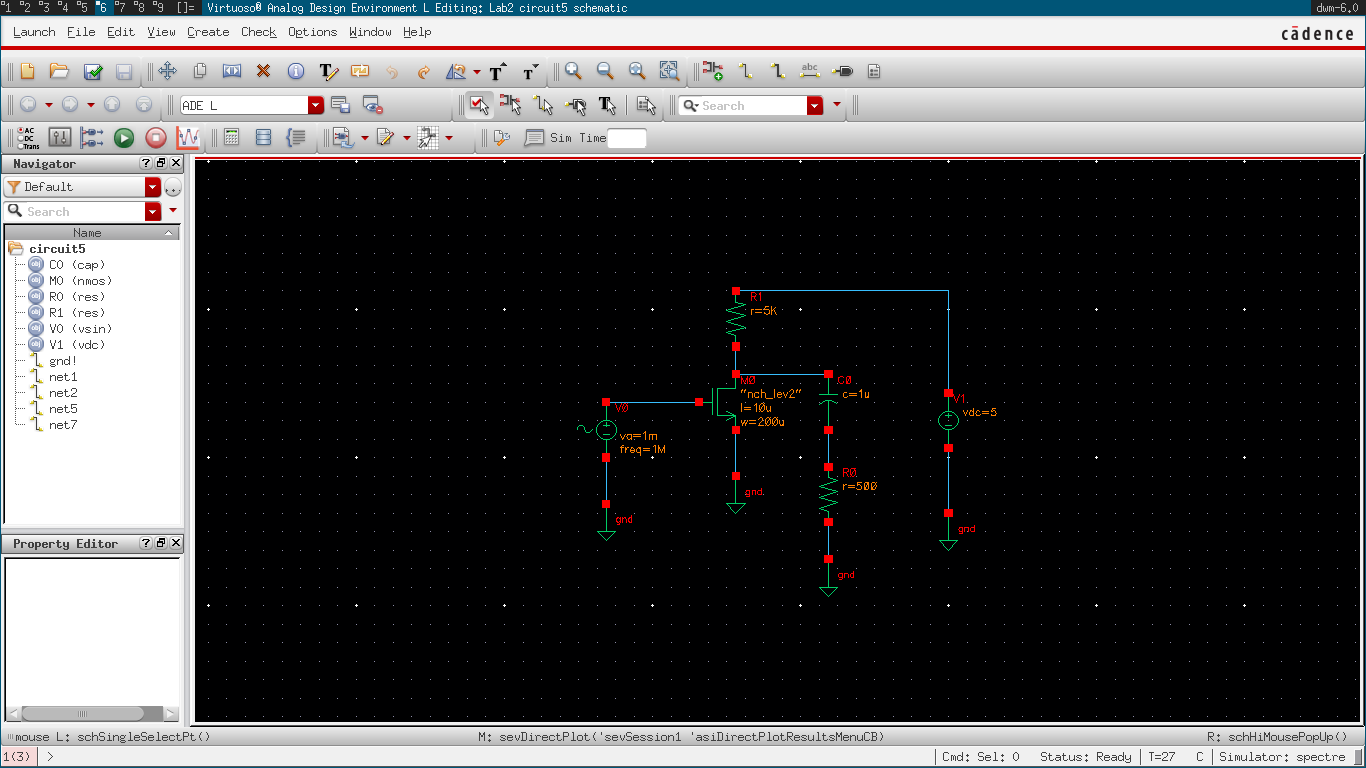
\includegraphics[scale=0.75]{../images/circuit5.PNG}
	\caption{Circuit 5}
	\label{fig:circuit5}
\end{figure}

\FloatBarrier

\FloatBarrier

\begin{figure}[h!]
	\centering
	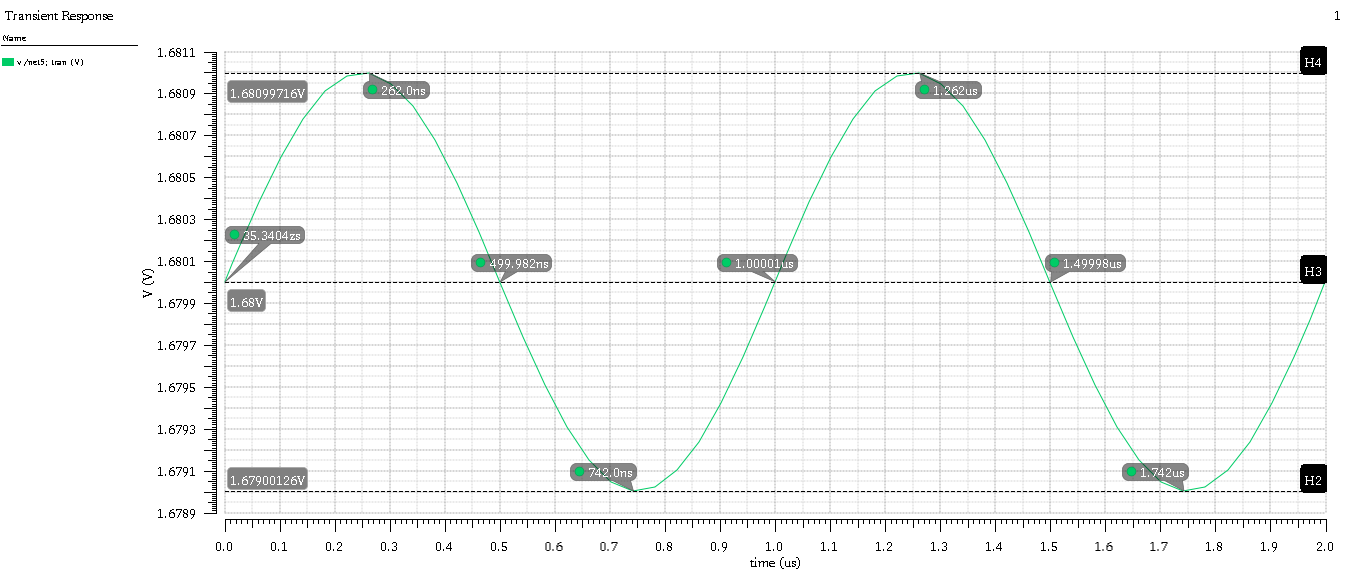
\includegraphics[scale=0.75]{../images/sim5_vin.PNG}
	\caption{$V_{in}$ for Small-Signal Test of Circuit 5}
	\label{fig:sim5_vin}
\end{figure}

\FloatBarrier

\FloatBarrier

\begin{figure}[h!]
	\centering
	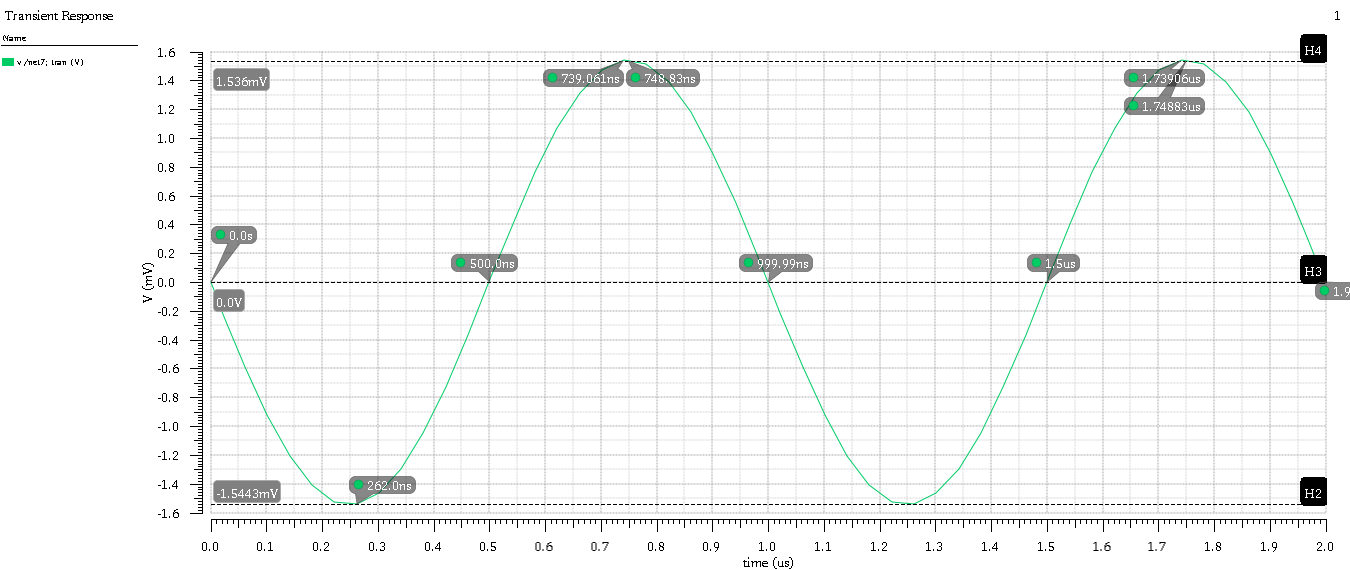
\includegraphics[scale=0.75]{../images/sim5_vout.PNG}
	\caption{$V_{out}$ for Small-Signal Test of Circuit 5}
	\label{fig:sim5_vout}
\end{figure}

\FloatBarrier

The small-signal gain can simply be acquired by taking the ratio of the amplitude of $V_{out}$ to the amplitude of $V_{in}$. This should also be multiplied by a factor of $-1$ since the signals are out of phase by $180^{o}$.
The gain can be determined theoretically from $-g_{m} ( R_{D} || R_{L} )$.

% Determine gain for Circuit 5

\FloatBarrier

\begin{table}[h!]
	\centering
	\caption{Common-Source Amplifier Gain}
	\label{tab:common_source_amp_gain}
	\csvautotabular{../tables/common_source_amp_gain.csv}
\end{table}

\FloatBarrier

% Determine gain for Circuit 6

\FloatBarrier

\begin{figure}[h!]
	\centering
	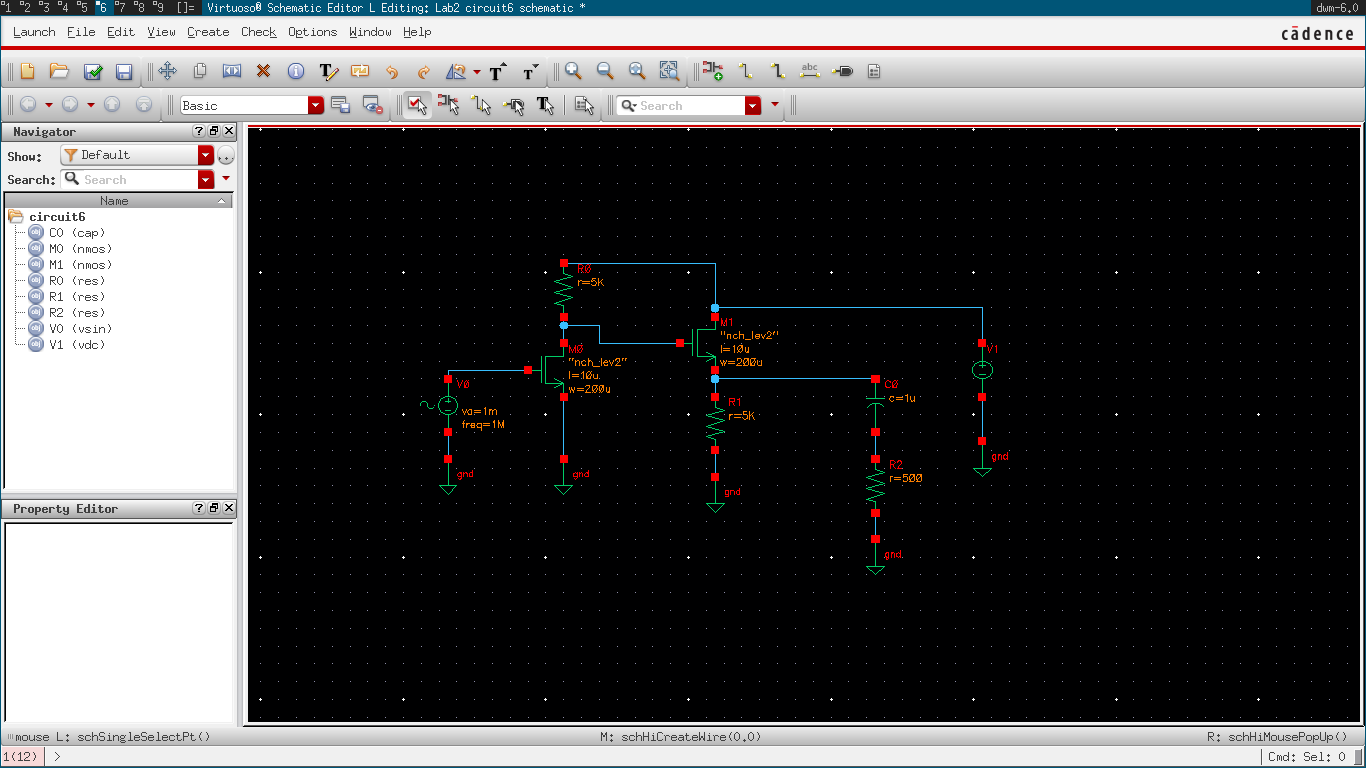
\includegraphics[scale=0.75]{../images/circuit6.PNG}
	\caption{Two-Stage Amplifier}
	\label{fig:circuit6}
\end{figure}

\FloatBarrier

The common-drain amplifier at the output will present nearly the same output voltage, but with a much lower output resistance.
The theoretical gain can be calculated by multiplying a common-source gain with a common-drain gain (assumed to be about 1) and then applying the voltage division equation.

\begin{equation}
	\label{eq:theoretical_cascaded_gain}
	A_{cascade} = -\frac{ g_{m,CSA} R_{D} R_{L} }{ r_{out,CDA} + R_{L} }
\end{equation}

\FloatBarrier

\begin{table}[h!]
	\centering
	\caption{Gain of Cascaded Amplifier}
	\label{tab:cascade_gain}
	\csvautotabular{../tables/cascade_gain.csv}
\end{table}

\FloatBarrier
